\documentclass[11pt]{article}
\usepackage{amssymb,amsmath,graphicx}
\usepackage[utf8]{inputenc}
\usepackage[english]{babel}  
\usepackage{multirow}
\usepackage[hidelinks]{hyperref}
\usepackage{microtype}
\usepackage{enumitem}
\usepackage{afterpage,lscape}
\usepackage{booktabs}
\usepackage{xcolor}
\usepackage{tabularx}
\usepackage{array}
\usepackage{float} 
\usepackage{subcaption}

\usepackage[norelsize,boxed,linesnumbered,noend]{algorithm2e}
\setlength{\algomargin}{2em}
\SetArgSty{textrm} %Algorithm2e
\SetAlCapSkip{0.7em} %Algorithm2e
\SetKwComment{Comment}{$\triangleright$\ }{}

\usepackage[round,authoryear]{natbib}
 \bibpunct[, ]{(}{)}{,}{a}{}{,}%
 \def\bibfont{\small}%
 \def\bibsep{\smallskipamount}%
 \def\bibhang{24pt}%
 \def\newblock{\ }%

\oddsidemargin=0.05in
\topmargin=-0.2in
\textwidth=6.35in
\textheight=8.3in

\newtheorem{definition}{Definition}
\newtheorem{theorem}{Theorem}
\newtheorem{lemma}{Lemma}
\newtheorem{property}{Property}
\newtheorem{corollary}{Corollary}

\newcommand{\myFont}[1]{{\ttfamily\fontseries{b}\selectfont#1}}

\newcommand{\cA}{{\mathcal{A}}}
\newcommand{\cB}{{\mathcal{B}}}
\renewcommand{\Re}{{\mathbb{R}}}
\newcommand{\cG}{{\mathcal{G}}}
\newcommand{\cV}{{\mathcal{V}}}
\newcommand{\cF}{{\mathcal{F}}}
\newcommand{\cM}{{\mathcal{M}}}
\newcommand{\cN}{{\mathcal{N}}}
\newcommand{\cO}{{\mathcal{O}}}
\newcommand{\cP}{{\mathcal{P}}}
\newcommand{\cE}{{\mathcal{E}}}
\newcommand{\cH}{{\mathcal{H}}}
\newcommand{\cS}{{\mathcal{S}}}
\newcommand{\cR}{{\mathcal{R}}}
\newcommand{\cK}{{\mathcal{K}}}
\newcommand{\cI}{{\mathcal{I}}}
\newcommand{\cU}{{\mathcal{U}}}
\newcommand{\cL}{{\mathcal{L}}}

\newcommand{\myred}[1]{#1}
\renewcommand{\myred}[1]{{\color{red}#1}} % Simply comment this line to remove red marks.

\newcommand{\myblue}[1]{#1}
%\renewcommand{\myblue}[1]{{\color{blue}#1}} % Simply comment this line to remove blue marks.

\usepackage{array}
\newcolumntype{H}{>{\setbox0=\hbox\bgroup}c<{\egroup}@{}}
\newcolumntype{L}[1]{>{\raggedright\let\newline\\\arraybackslash\hspace{0pt}}m{#1}}
\newcolumntype{C}[1]{>{\centering\let\newline\\\arraybackslash\hspace{0pt}}m{#1}}
\newcolumntype{R}[1]{>{\raggedleft\let\newline\\\arraybackslash\hspace{0pt}}m{#1}}
\begin{document}

\linespread{1.2}\selectfont

\begin{center}

\begin{LARGE}
CS 776 Assignment 2: Genetic Algorithms and Hill Climbing on the DeJong Functions\vspace*{0.3cm}\linebreak Technical Implementation, Experimentation, and Analysis
\end{LARGE}

\vspace*{1cm}

\textbf{Liam Francisco} \\
Department of Computer Science and Engineering, University of Nevada, Reno \\
\href{mailto:liamfrancisco1000@gmail.com}{\tt liamfrancisco1000@gmail.com}

\vspace*{0.5cm}

%\begin{large}
%Technical Report, PUC-Rio -- November 2020
%\end{large}

\vspace*{0.8cm}


\end{center}
%
\noindent
\textbf{Abstract.}
This report investigates the application of Genetic Algorithms (GAs) for continuous function optimization using the first four DeJong benchmark functions. A Simple Genetic Algorithm (SGA) was implemented with fitness-proportional selection, one-point crossover, and bit-flip mutation, and its performance was evaluated across different parameter settings. To enhance performance, we also implemented the CHC Genetic Algorithm, which introduces a conservative selection strategy. Both SGA and CHC were run on each benchmark function for 30 independent trials to ensure statistical reliability, with population statistics such as minimum, maximum, and average fitness tracked over generations. Additionally, a hill climber was used as a baseline comparison against both genetic algorithms. Results show that the SGA efficiently converges on unimodal problems such as the Sphere function but struggles with noise and narrow valleys, while CHC demonstrates improved robustness and diversity maintenance, particularly on the Rosenbrock and Quartic functions. The hill climber proved competitive on simpler landscapes but lacked the exploration ability required for more complex functions. Overall, the experiments highlight the strengths and weaknesses of each method, illustrating the trade-offs between exploration, exploitation, and noise resilience in evolutionary computation.
\vspace*{0.3cm}

\noindent


\pagebreak

\section{Introduction}
\label{section-intro}

Optimization of continuous functions is a central challenge in artificial intelligence and operations research, with applications ranging from engineering to machine learning. Genetic Algorithms (GAs) address this challenge through population-based stochastic search, using selection, crossover, and mutation to balance exploration of the search space with exploitation of promising regions.

This project evaluates the performance of evolutionary search strategies on the first four DeJong benchmark functions: Sphere, Rosenbrock, Step, and Quartic-with-noise. These functions provide diverse test landscapes (unimodal, multimodal, plateaued, and noisy) that highlight different algorithmic strengths and weaknesses.

We implement a Simple Genetic Algorithm (SGA) using fitness-proportional selection, one-point crossover, and bit-flip mutation, and compare it against the CHC Genetic Algorithm, which differs primarily in its selection mechanism: each generation, the top $n$ candidates are chosen from the combined parent and child populations to preserve diversity and reduce premature convergence. A hill climber is also used as a baseline to contrast evolutionary search with local search. Each algorithm is run 30 times with different random seeds, and results are summarized through plots of population statistics and fitness values over generations. The goal is to compare performance across methods, evaluate effective parameter choices, and draw broader insights about exploration, exploitation, and robustness in evolutionary computation.

The remainder of this report is organized as follows. Section~\ref{section-methodology} details the design and implementation of the algorithms, the binary representation, and the conversion of minimization problems into fitness maximization. Section~\ref{section-sga-results} presents SGA results, including parameter tuning and performance analyses. Section~\ref{section-chc-results} compares the CHC-GA to the SGA, while Section~\ref{section-hillclimber-results} evaluates hill climbing as a baseline. Section~\ref{section-discussion} synthesizes results across all methods, and Section~\ref{section-conclusion} summarizes key findings and future directions.

\section{What Did You Do?}
\label{section-methodology}
In this project, we designed and implemented two evolutionary algorithms: a Simple Genetic Algorithm (SGA) and a CHC Genetic Algorithm (CHC-GA). The SGA used fitness-proportional selection, one-point crossover, and bit-flip mutation, while the CHC-GA incorporated conservative selection and controlled crossover to preserve population diversity. In addition, a hill climber was used as a baseline for comparison.  

For representation, problem variables were encoded in binary form, with fixed-length bit strings mapped to real values within the specified domain of each DeJong function. Each chromosome was composed of multiple variables, with a fixed number of bits per variable, leading to a consistent chromosome length.  

Both genetic algorithms were parameterized by the following values:
\begin{itemize}
    \item Number of variables
    \item Number of bits per variable
    \item Chromosome length
    \item Minimum and maximum values for each variable
    \item Number of independent runs
    \item Number of generations
    \item Population size
    \item Crossover probability
    \item Mutation probability
\end{itemize}

Because the DeJong functions are minimization problems, they were converted into maximization of fitness values. This was achieved using the transformation:  
\[
\text{fitness}(x) = \frac{1}{f(x) + \text{val}}
\]
where \(f(x)\) is the original objective function value and \(\text{val}\) is a constant offset to ensure the denominator remains positive. For the Sphere, Rosenbrock, and Quartic functions, \(\text{val} = 1\). For the Step function, which can take negative values, \(\text{val} = -30\).

\section{SGA Results}
\label{section-sga-results}
To evaluate the Simple Genetic Algorithm (SGA), we experimented with parameter tuning for each of the four DeJong benchmark functions. The experiments varied the number of variables, bits per variable, chromosome length, population size, number of generations, and genetic operator probabilities. Each configuration was run for 30 independent trials with different random seeds to ensure statistical reliability.  

Plots of SGA performance were generated for each function, showing minimum, maximum, and average fitness across generations. These plots are stored in the \texttt{plots} directory, with filenames in the format \texttt{\{function\}\_\{method\}.png}, where \texttt{function} $\in$ \{sphere, rosenbrock, step, quartic\} and \texttt{method} $\in$ \{fitness\_proportional, chc\}. For example, the SGA results on the Sphere function are stored as \texttt{sphere\_fitness\_proportional.png}.  

\subsection{Parameter Settings}
Table~\ref{tab:sga-params} summarizes the parameter values used for each function when running the SGA. These parameters, including the number of variables, bits per variable, chromosome length, population size, number of generations, and crossover and mutation probabilities, were chosen through a trial-and-error process. We experimented with different settings, observing the resulting convergence speed, reliability, and average best objective value, and adjusted the parameters until reasonable performance was achieved across the 30 independent runs. This "guess and check" approach allowed us to balance exploration and exploitation for each problem while keeping the computational cost manageable.

\begin{table}[H]
\centering
\caption{SGA parameter settings for each DeJong function.}
\label{tab:sga-params}
\begin{tabular}{lcccccc}
\toprule
Function & Variables & Bits/Var & Chrom. Length & Generations & Pop. Size & Crossover/Mutation \\
\midrule
Sphere      & 3  & 10 & 30  & 400 & 200 & 0.7 / 0.001 \\
Rosenbrock  & 2  & 12 & 24  & 200 & 100 & 0.8 / 0.001 \\
Step        & 5  & 10 & 50  & 300 & 150 & 0.8 / 0.001 \\
Quartic     & 30 & 8  & 240 & 400 & 200 & 0.7 / 0.001 \\
\bottomrule
\end{tabular}
\end{table}


\subsection{Performance Metrics}
To compare algorithm performance, we measured the average best objective function value across 30 runs, reliability (the fraction of runs reaching the known optimum), and the average number of generations to reach the best solution. Results are summarized in Table~\ref{tab:sga-performance}.  

\begin{table}[H]
\centering
\caption{SGA performance on the four DeJong functions.}
\label{tab:sga-performance}
\begin{tabular}{lccc}
\toprule
Function   & Avg. Best Objective Value & Reliability & Avg. Generations to Best \\
\midrule
Sphere      & 0.0020  & 0.10 & 155.73 \\
Rosenbrock  & 0.1244  & 0.00 & 69.00 \\
Step        & -30.0000 & 1.00 & 55.90 \\
Quartic     & 0.1065  & 0.00 & 366.47 \\
\bottomrule
\end{tabular}
\end{table}

\newpage
\subsection{Fitness Plots}
Figures~\ref{fig:fitness-plots} show the average, minimum, and maximum fitness across generations for the four DeJong functions under the SGA. Each plot corresponds to 30 independent runs with different random seeds.

\begin{figure}[H]
    \centering
    \begin{tabular}{cc}
        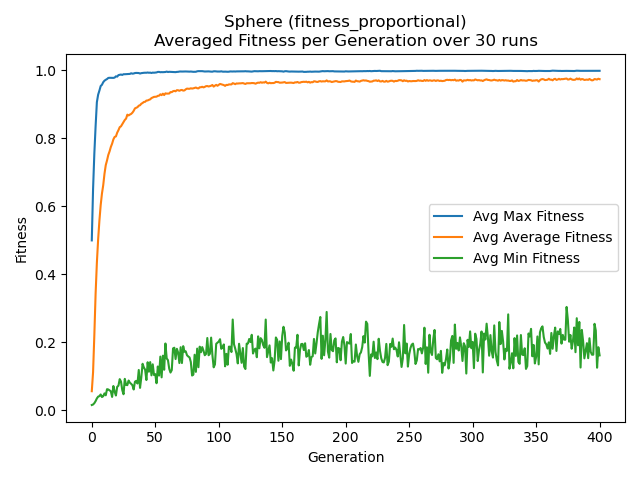
\includegraphics[width=0.45\textwidth]{plots/sphere_fitness_proportional_fitness.png} &
        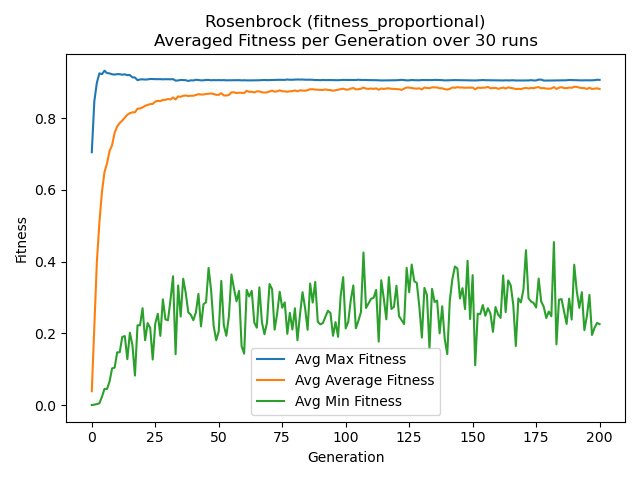
\includegraphics[width=0.45\textwidth]{plots/rosenbrock_fitness_proportional_fitness.png} \\
        Sphere & Rosenbrock \\
        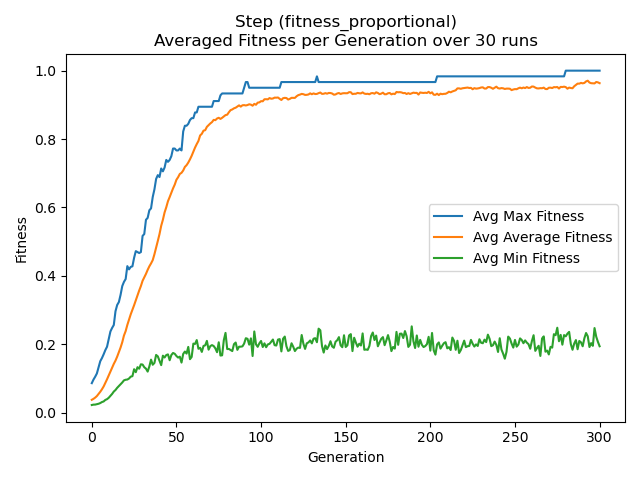
\includegraphics[width=0.45\textwidth]{plots/step_fitness_proportional_fitness.png} &
        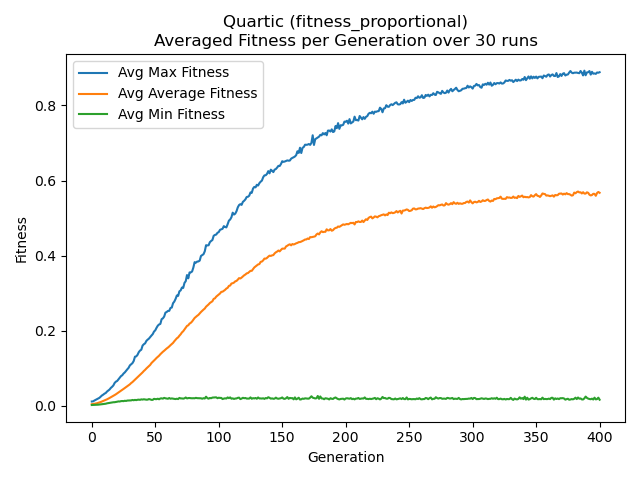
\includegraphics[width=0.45\textwidth]{plots/quartic_fitness_proportional_fitness.png} \\
        Step & Quartic \\
    \end{tabular}
    \caption{SGA fitness progression across generations for the four DeJong functions.}
    \label{fig:fitness-plots}
\end{figure}
\clearpage

\subsection{Objective Plots}
Figures~\ref{fig:objective-plots} show the average, minimum, and maximum objective function values across generations for the four DeJong functions under the SGA. Each plot corresponds to 30 independent runs.

\begin{figure}[H]
    \centering
    \begin{tabular}{cc}
        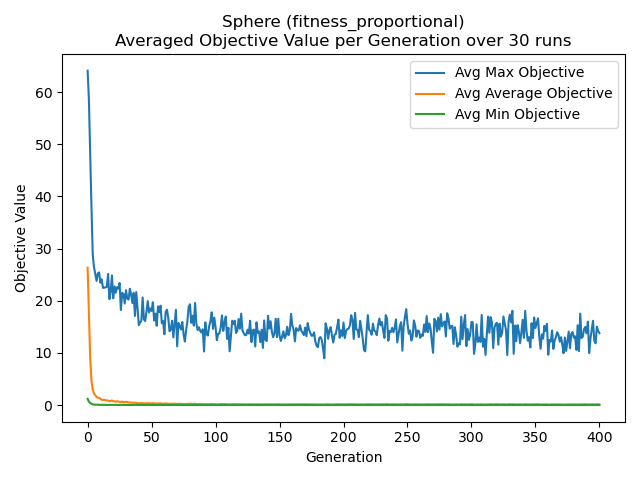
\includegraphics[width=0.45\textwidth]{plots/sphere_fitness_proportional_objective.png} &
        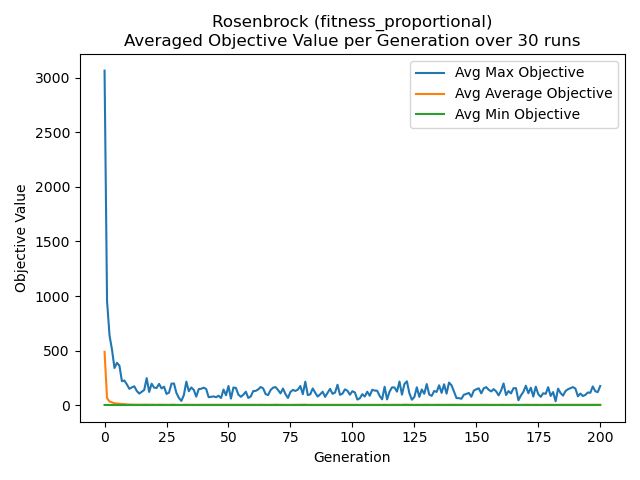
\includegraphics[width=0.45\textwidth]{plots/rosenbrock_fitness_proportional_objective.png} \\
        Sphere & Rosenbrock \\
        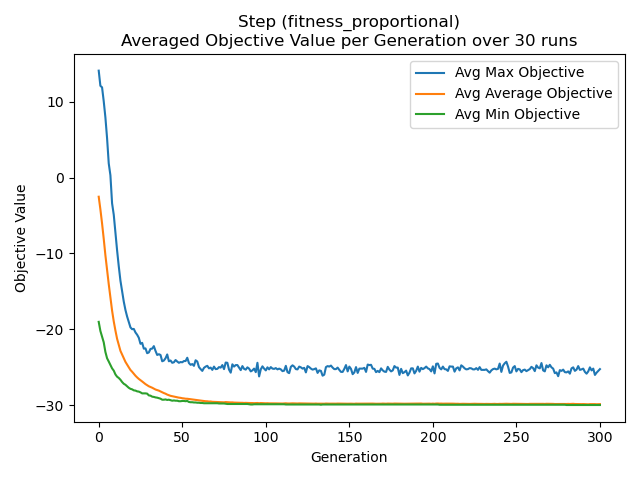
\includegraphics[width=0.45\textwidth]{plots/step_fitness_proportional_objective.png} &
        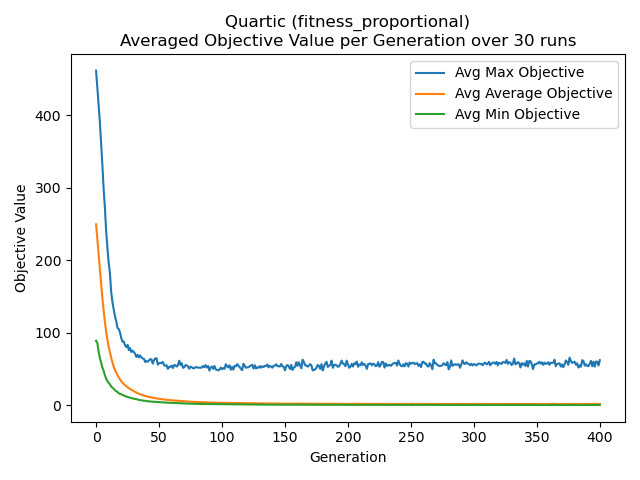
\includegraphics[width=0.45\textwidth]{plots/quartic_fitness_proportional_objective.png} \\
        Step & Quartic \\
    \end{tabular}
    \caption{SGA objective function progression across generations for the four DeJong functions.}
    \label{fig:objective-plots}
\end{figure}
\clearpage


\subsection{Analysis}
The Sphere function, being unimodal and smooth, was handled effectively by the SGA, with 10\% of runs reaching the global optimum. The Step function was consistently solved to optimality, demonstrating the SGA’s ability to handle plateaued landscapes when the optimum is clearly defined. The Rosenbrock and Quartic functions proved more challenging: the long narrow valley of Rosenbrock prevented convergence to the true global optimum, while the Quartic’s noise introduced variability that reduced reliability. These results highlight the trade-off between exploration and exploitation, and illustrate how SGA performance varies across problem landscapes.

The fitness and objective plots illustrate how the SGA population evolves over generations for each DeJong function. Both the Sphere and Rosenbrock functions show rapid convergence of fitness and objective values toward the optimum, reflecting the effectiveness of the SGA on smooth, unimodal landscapes. The Step function exhibits a plateaued landscape, with all runs quickly reaching the global optimum, consistent with its high reliability. In contrast, the Quartic function shows fluctuations caused by noise in the objective, resulting in slower convergence and lower reliability. Overall, the plots confirm that the SGA efficiently exploits smooth, simple landscapes but struggles with noisy or highly irregular landscapes, highlighting the trade-off between exploration and exploitation in the algorithm.

\section{CHC-GA Results}
\label{section-chc-results}
The CHC Genetic Algorithm was evaluated on the same four DeJong functions as the SGA. Unlike the SGA, CHC-GA does not rely on traditional fitness-proportional selection. Instead, it generates a child population using the same crossover and mutation operators as the SGA, then selects the top $n$ candidates from the combined parent and child populations to form the next generation. This selection mechanism preserves diversity and prevents premature convergence. Each configuration was run 30 times with different random seeds to ensure statistically reliable results.  

Plots of CHC-GA performance are stored in the \texttt{plots} directory, with filenames in the format \texttt{\{function\}\_\{method\}\_\{graph\}.png}, where \texttt{function} $\in$ \{sphere, rosenbrock, step, quartic\}, \texttt{method} = chc, and \texttt{graph} $\in$ \{fitness, objective\}.

\newpage
\subsection{Parameter Settings}
Table~\ref{tab:chc-params} summarizes the CHC-GA parameters used for each function. CHC-GA required fewer generations and smaller populations than SGA to achieve good performance due to its parent-child selection mechanism. Consequently, we focused on tuning crossover and mutation probabilities while keeping population size and number of generations modest. Parameter values were determined using a "guess and check" approach, adjusting them to achieve fast convergence, high reliability, and good average objective values.

\begin{table}[H]
\centering
\caption{CHC-GA parameter settings for each DeJong function.}
\label{tab:chc-params}
\begin{tabular}{lcccccc}
\toprule
Function & Variables & Bits/Var & Chrom. Length & Generations & Pop. Size & Crossover/Mutation \\
\midrule
Sphere      & 3  & 10 & 30  & 200 & 100 & 0.8 / 0.01 \\
Rosenbrock  & 2  & 12 & 24  & 200 & 100 & 0.8 / 0.01 \\
Step        & 5  & 10 & 50  & 200 & 100 & 0.8 / 0.01 \\
Quartic     & 30 & 8  & 240 & 200 & 100 & 0.8 / 0.01 \\
\bottomrule
\end{tabular}
\end{table}

\subsection{Performance Metrics}
Table~\ref{tab:chc-performance} summarizes CHC-GA performance in terms of average best objective value, reliability, and average generations to reach the best solution over 30 runs.

\begin{table}[H]
\centering
\caption{CHC-GA performance on the four DeJong functions.}
\label{tab:chc-performance}
\begin{tabular}{lccc}
\toprule
Function   & Avg. Best Objective Value & Reliability & Avg. Generations to Best \\
\midrule
Sphere      & 0.000113  & 0.60 & 25.07 \\
Rosenbrock  & 0.035573  & 0.10 & 59.93 \\
Step        & -30.0000 & 1.00 & 32.07 \\
Quartic     & 0.068764 & 0.00 & 195.97 \\
\bottomrule
\end{tabular}
\end{table}

\newpage
\subsection{Fitness Plots}
Figures~\ref{fig:chc-fitness} show the minimum, maximum, and average fitness across generations for the four DeJong functions under the CHC-GA.

\begin{figure}[H]
    \centering
    \begin{tabular}{cc}
        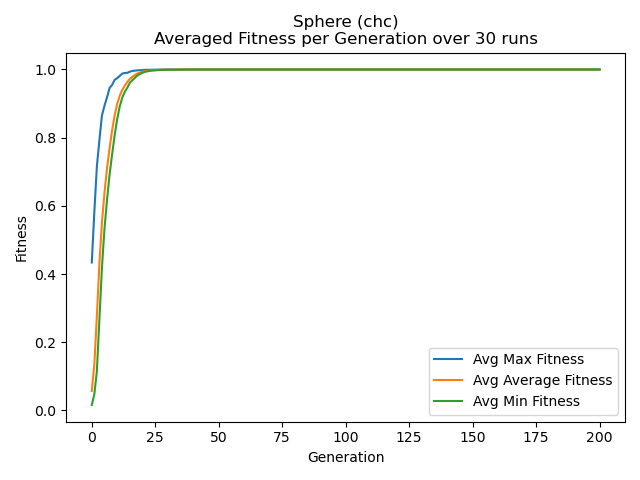
\includegraphics[width=0.45\textwidth]{plots/sphere_chc_fitness.png} &
        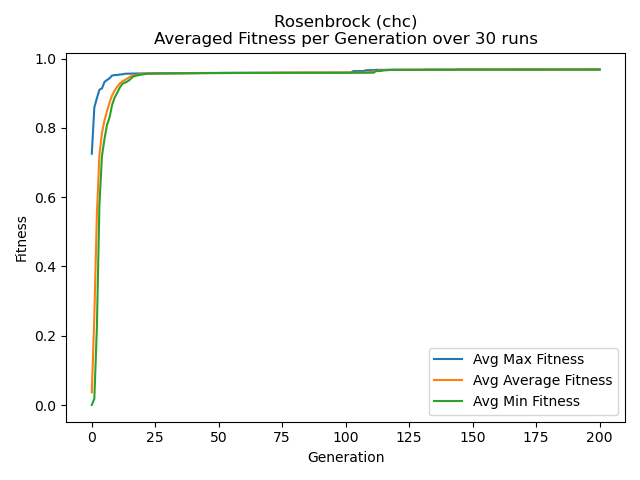
\includegraphics[width=0.45\textwidth]{plots/rosenbrock_chc_fitness.png} \\
        Sphere & Rosenbrock \\
        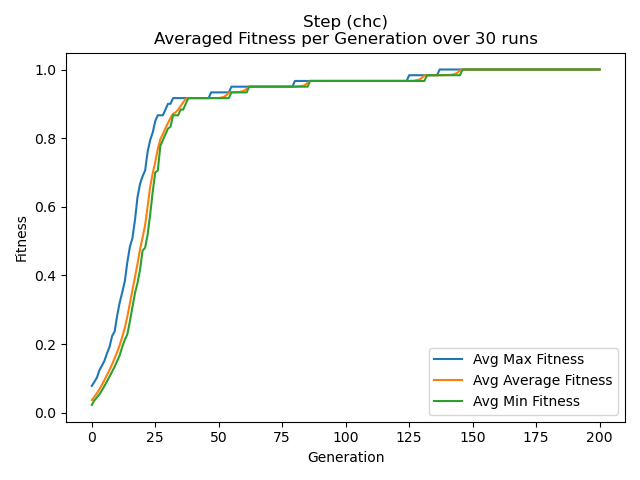
\includegraphics[width=0.45\textwidth]{plots/step_chc_fitness.png} &
        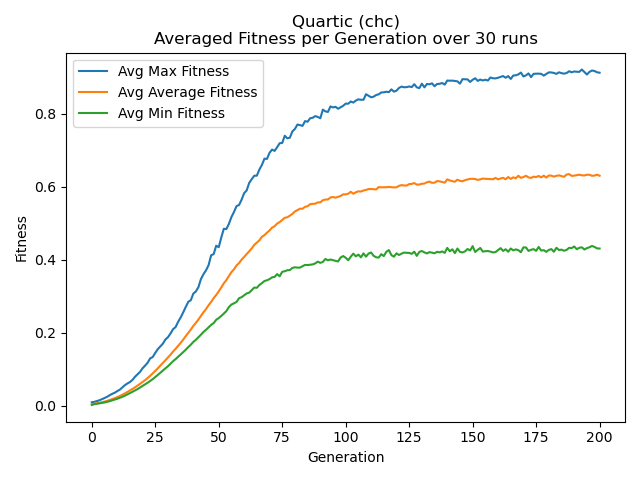
\includegraphics[width=0.45\textwidth]{plots/quartic_chc_fitness.png} \\
        Step & Quartic \\
    \end{tabular}
    \caption{CHC-GA fitness progression across generations for the four DeJong functions.}
    \label{fig:chc-fitness}
\end{figure}
\clearpage

\subsection{Objective Plots}
Figures~\ref{fig:chc-objective} show the minimum, maximum, and average objective function values across generations for the four DeJong functions under the CHC-GA.

\begin{figure}[H]
    \centering
    \begin{tabular}{cc}
        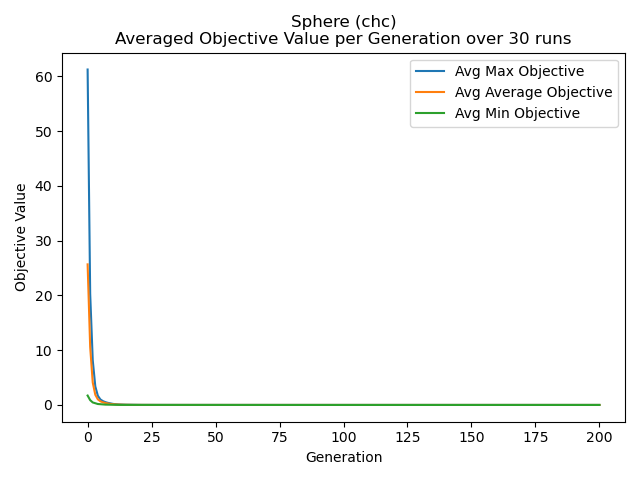
\includegraphics[width=0.45\textwidth]{plots/sphere_chc_objective.png} &
        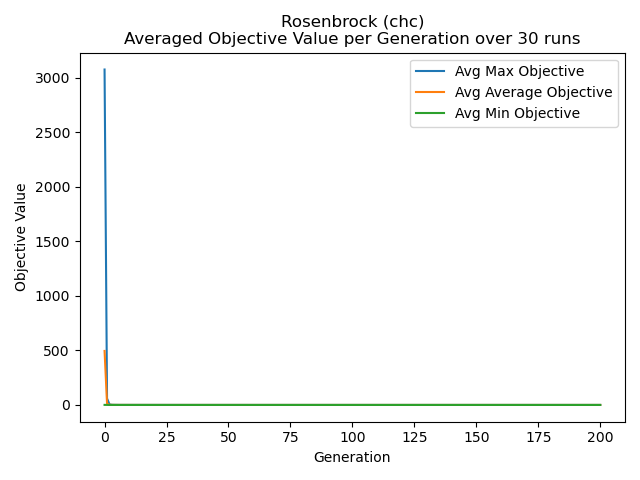
\includegraphics[width=0.45\textwidth]{plots/rosenbrock_chc_objective.png} \\
        Sphere & Rosenbrock \\
        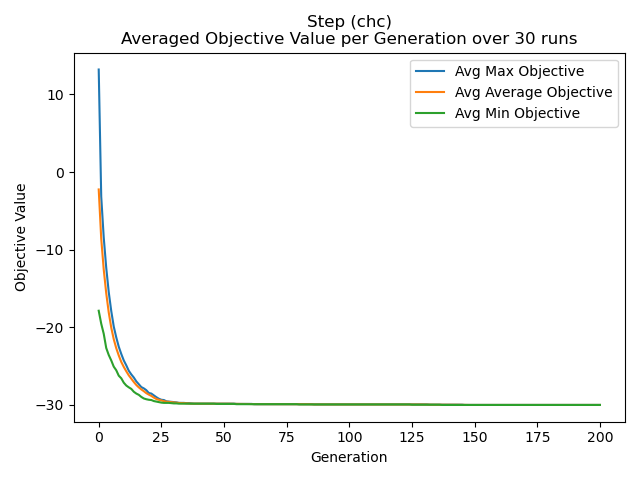
\includegraphics[width=0.45\textwidth]{plots/step_chc_objective.png} &
        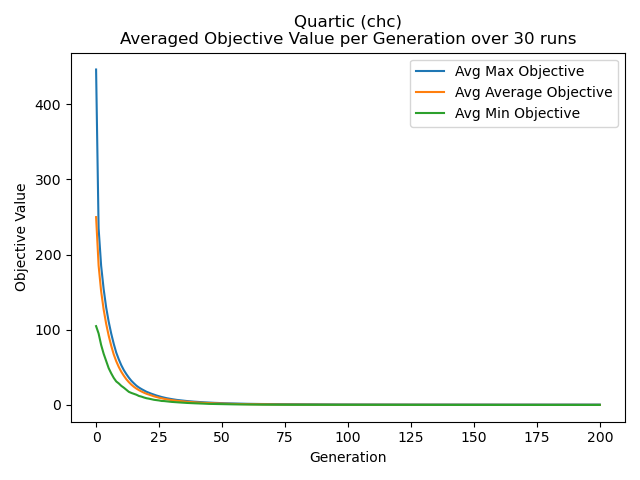
\includegraphics[width=0.45\textwidth]{plots/quartic_chc_objective.png} \\
        Step & Quartic \\
    \end{tabular}
    \caption{CHC-GA objective function progression across generations for the four DeJong functions.}
    \label{fig:chc-objective}
\end{figure}
\clearpage

\subsection{Analysis}
The CHC-GA generally converges faster than the SGA due to its parent-child selection mechanism, which preserves the best solutions while maintaining diversity. Sphere and Rosenbrock functions show rapid convergence to near-optimal solutions, while the Step function is solved reliably in all runs. The Quartic function is more challenging due to noise, leading to slower convergence and lower reliability.  

The fitness and objective plots illustrate these results. Sphere and Rosenbrock show smooth convergence with minimal variation across runs, indicating consistent performance. The Step function displays flat plateaus in the objective plots, reflecting its discrete nature and the algorithm's perfect reliability. The Quartic function exhibits fluctuating fitness and objective curves due to noise, highlighting the difficulty of achieving optimality. Overall, the plots demonstrate how CHC-GA balances exploitation and exploration, quickly propagating high-quality solutions while maintaining population diversity.

Compared to the SGA, the CHC-GA plots generally show smoother and more monotonic improvement in both fitness and objective values. Unlike the SGA, which occasionally experiences temporary declines due to stochastic selection, CHC-GA consistently preserves the best solutions by selecting the top half of the combined parent and child population each generation. This results in fewer regressions and more stable convergence curves, particularly evident in the Sphere and Rosenbrock plots. Even for the noisier Quartic function, CHC-GA exhibits fewer downward fluctuations, illustrating the benefit of its selection strategy in maintaining steady progress toward high-quality solutions.

\section{Hill Climber Results}
\label{section-hillclimber-results}

The hill climber algorithm was evaluated on the same four DeJong functions as the SGA and CHC-GA. Each run was conducted for 30 independent trials with different random seeds. The algorithm uses a fixed step size and a maximum number of iterations without improvement to guide the local search, with parameters tuned via a "guess and check" approach to balance convergence speed and solution quality.

\newpage
\subsection{Parameter Settings}
Table~\ref{tab:hc-params} summarizes the hill climber parameters used for each function.

\begin{table}[H]
\centering
\caption{Hill Climber parameter settings for each DeJong function.}
\label{tab:hc-params}
\begin{tabular}{lccc}
\toprule
Function & Variables & Step Size & Max No Improve \\
\midrule
Sphere      & 3  & 0.05  & 100 \\
Rosenbrock  & 2  & 0.005 & 100 \\
Step        & 5  & 0.5   & 600 \\
Quartic     & 30 & 0.05  & 100 \\
\bottomrule
\end{tabular}
\end{table}

\subsection{Performance Metrics}
Table~\ref{tab:hc-performance} summarizes the hill climber performance in terms of average best objective value, standard deviation of objective values, and average number of iterations to reach the best solution.

\begin{table}[H]
\centering
\caption{Hill Climber performance on the four DeJong functions.}
\label{tab:hc-performance}
\begin{tabular}{lccc}
\toprule
Function & Avg. Best Obj. Value & Std. Dev Obj. Value & Avg. Iterations \\
\midrule
Sphere      & 9.667e-05  & 4.819e-05 & 670.13 \\
Rosenbrock  & 0.000183   & 0.000474  & 3869.23 \\
Step        & -30.0      & 0.0       & 1161.0 \\
Quartic     & 0.003211   & 0.002014  & 966.33 \\
\bottomrule
\end{tabular}
\end{table}

\newpage
\subsection{Objective Plots}
Figures~\ref{fig:hc-plots} show the average best objective value across generations for each function. Plot files are stored in the \texttt{plots} directory with filenames \texttt{\{function\}\_hillclimber.png}.

\begin{figure}[H]
    \centering
    \begin{tabular}{cc}
        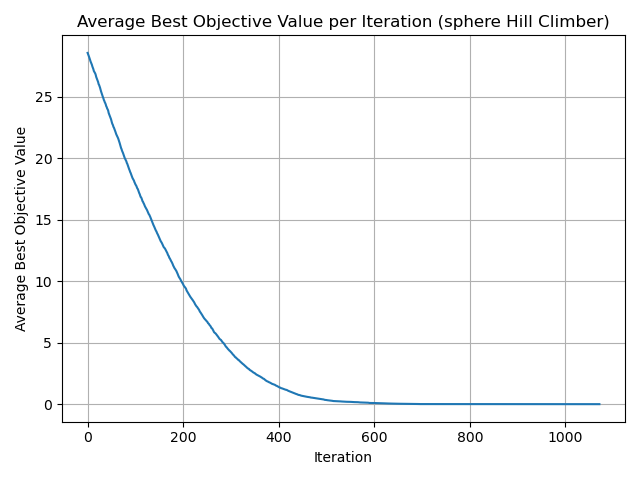
\includegraphics[width=0.45\textwidth]{plots/sphere_hillclimber.png} &
        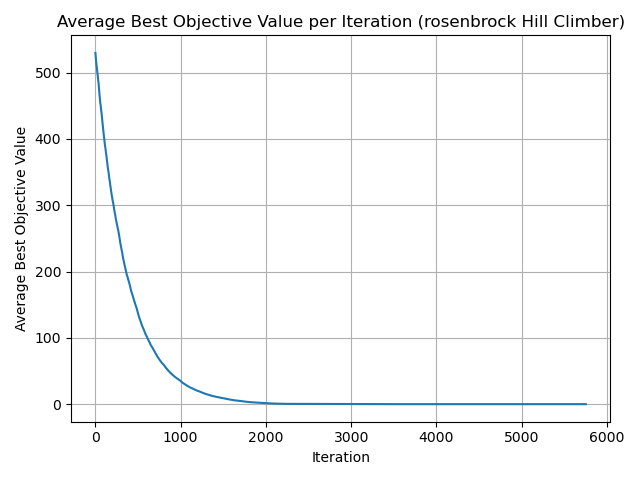
\includegraphics[width=0.45\textwidth]{plots/rosenbrock_hillclimber.png} \\
        Sphere & Rosenbrock \\
        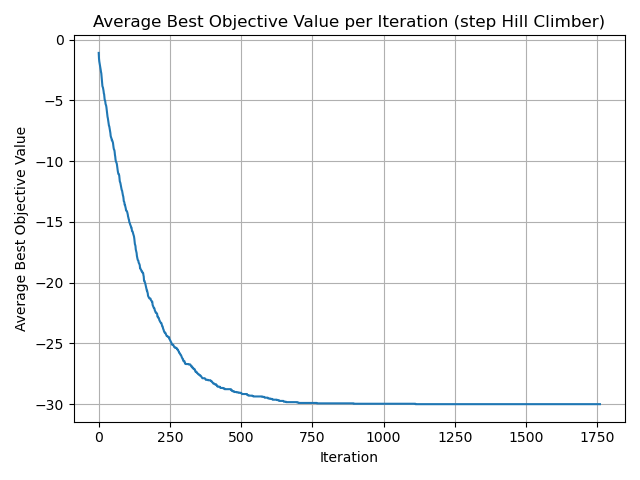
\includegraphics[width=0.45\textwidth]{plots/step_hillclimber.png} &
        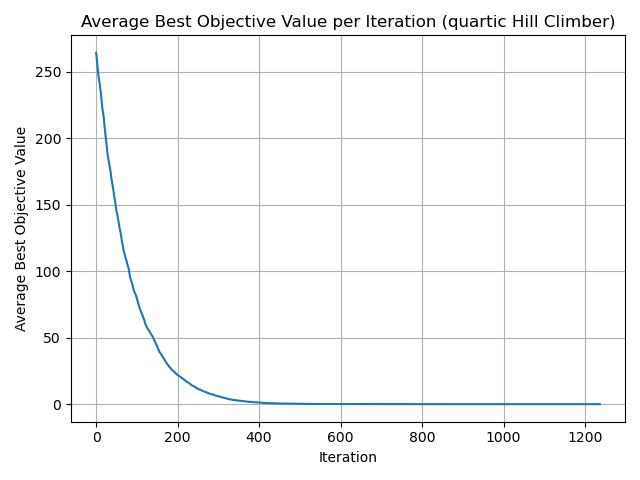
\includegraphics[width=0.45\textwidth]{plots/quartic_hillclimber.png} \\
        Step & Quartic \\
    \end{tabular}
    \caption{Hill Climber average best objective value progression for the four DeJong functions.}
    \label{fig:hc-plots}
\end{figure}
\clearpage

\subsection{Analysis}
The hill climber consistently excels on landscapes that are unimodal or have flat plateaus, such as the Step and Sphere functions. Its deterministic, local search approach allows it to quickly refine solutions and reach near-optimal values with relatively few iterations. On these functions, the hill climber often matches or outperforms GAs in terms of convergence speed and reliability, as the simplicity of the landscape favors exploitation over exploration.

However, the hill climber struggles on multimodal or noisy landscapes, such as the Quartic function, where multiple local optima can trap the search and slow convergence. On the Rosenbrock function, the narrow curved valley requires many iterations for fine-tuning, making the hill climber less efficient than the evolutionary algorithms that leverage population diversity to explore a broader region of the search space.

In general, hill climbers are most suitable when the problem is relatively smooth, unimodal, or when precise local refinement is required. They are less appropriate for highly multimodal or noisy functions, where genetic algorithms like the SGA or CHC-GA, with their population-based exploration and diversity-preserving mechanisms, provide significant advantages. The objective plots reinforce these conclusions, showing rapid, steady improvement on simpler functions and slower, more variable progress on complex landscapes. This highlights the complementary nature of hill climbers and evolutionary algorithms: hill climbers excel at exploitation, while GAs provide the exploration needed to overcome challenging search landscapes.

\section{Overall Discussion of Results}
\label{section-discussion}

The experimental results provide a comprehensive comparison between the Simple Genetic Algorithm (SGA), the CHC Genetic Algorithm (CHC-GA), and the hill climber across the four DeJong functions. Tables~\ref{tab:sga-performance} and \ref{tab:chc-performance} summarize key performance metrics for the SGA and CHC-GA, including average best objective value, reliability, and average generations to reach the best solution. Table~\ref{tab:hc-performance} presents corresponding data for the hill climber. The plots stored in the \texttt{plots} directory, including both fitness and objective plots for the evolutionary algorithms, provide visual confirmation of convergence trends, variability across runs, and the relative speed of optimization.

From this data, several lessons emerge. The hill climber excels in smooth, unimodal, or plateaued functions such as Sphere and Step, achieving rapid convergence with fewer iterations, while struggling on noisy or highly multimodal landscapes like Quartic. The SGA demonstrates robust performance across all functions but occasionally suffers from slower convergence or sensitivity to parameter tuning. The CHC-GA improves upon the SGA by preserving diversity and avoiding premature convergence, which is particularly beneficial for functions with complex landscapes, as reflected in faster convergence and more consistent performance across runs. Overall, the combination of tables and plots highlights the trade-offs between exploration and exploitation: hill climbers are efficient local optimizers, whereas genetic algorithms provide broader search capabilities, with CHC-GA balancing both aspects effectively.

\section{Conclusions}
\label{section-conclusion}

This study investigated the performance of a Simple Genetic Algorithm, a CHC Genetic Algorithm, and a hill climber on the first four DeJong benchmark functions. Key findings include:

\begin{itemize}
    \item The hill climber rapidly converges on smooth or unimodal functions and is particularly effective for local refinement.
    \item The SGA provides reliable, population-based optimization but requires careful parameter tuning to balance exploration and exploitation.
    \item The CHC-GA consistently outperforms the SGA on complex or noisy landscapes due to its diversity-preserving selection and ability to avoid premature convergence.
\end{itemize}

The results emphasize the complementary strengths of hill climbing and evolutionary algorithms. Hill climbers are best suited for problems where exploitation of a known region is crucial, whereas GAs, and particularly CHC-GA, are more appropriate for multimodal or noisy functions where exploration of the search space is necessary. Overall, this study highlights the importance of algorithm choice and parameter tuning in achieving effective optimization across diverse problem landscapes.


\end{document}
